% \documentclass{article}

% \usepackage[utf8]{inputenc} 
% \usepackage[french]{babel} 
% \usepackage{portland} 
% \usepackage{epsfig} 
% \usepackage{url} 
% \usepackage{hyperref} 
% \usepackage{fancybox} 
% \usepackage{pgf}

% \pgfdeclareimage[height=12cm]{arbre}{arbre}
% \pgfdeclareimage[width=\textwidth]{automate}{automate}

% %\newtheorem{exemple}{Exemple} 
% \newtheorem{definition}{D{\'e}finition} 
% %\newtheorem{remarque}{Remarque} 
% %\newtheorem{question}{Question} 
% %\newtheorem{notation}{Notation} 
% %\newtheorem{remarques}{Remarques} 

% \title{Grep : construire l'automate}

% \begin{document}
% \maketitle


\section{Construction d'un automate non d{\'e}terministe {\`a} partir d'un arbre de syntaxe abstraite}

Illustrons la m{\'e}thode {\`a} l'aide d'un exemple. Consid\'erons l'expression rationnelle~: 
\[ (ab+c)^\star ab \] correspondant {\`a} l'arbre de syntaxe de la Figure~\ref{as} page~\pageref{as}. 
Le but de l'algorithme est de construire l'automate de la Figure~\ref{au} page~\pageref{au}.
\begin{figure}
\begin{center}
  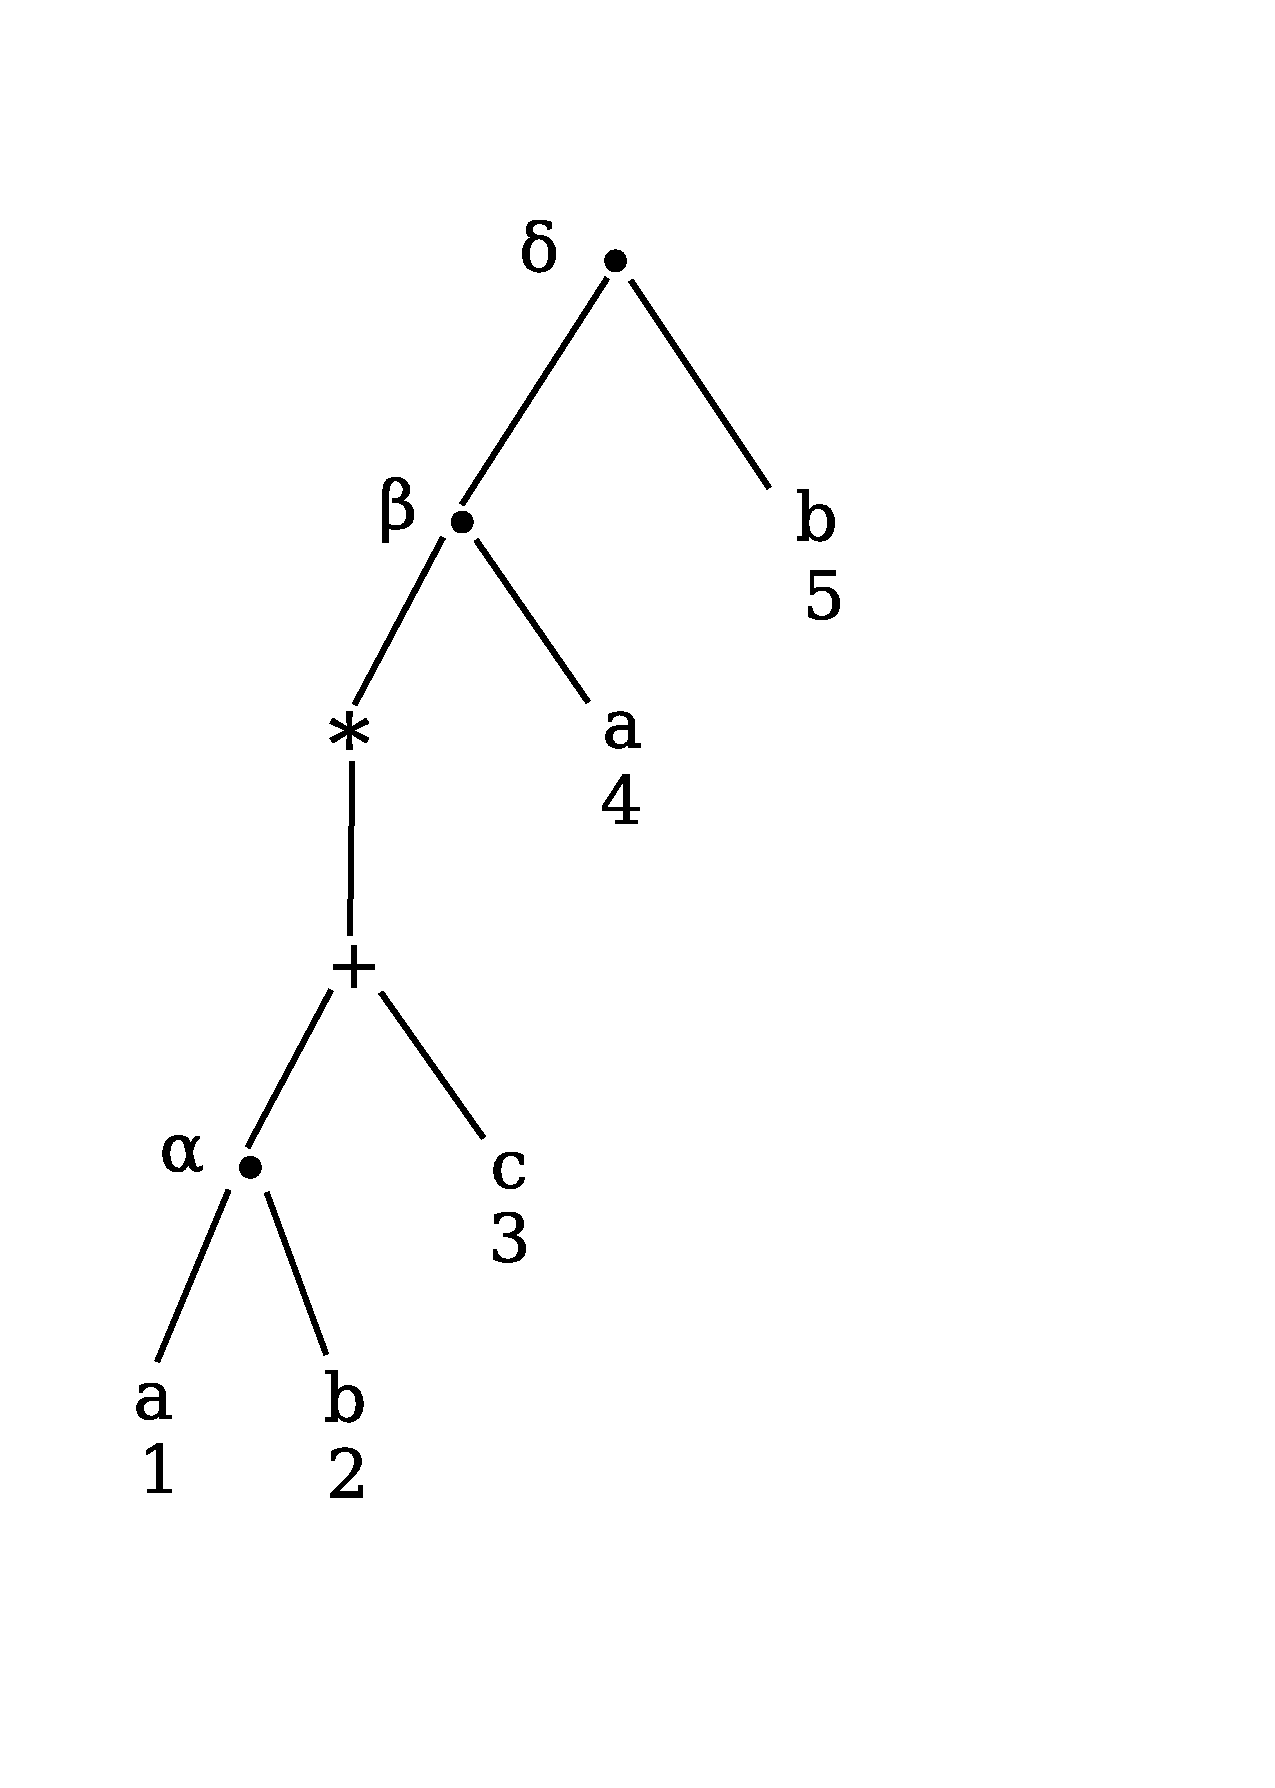
\includegraphics[width=5cm]{arbre}
%\pgfuseimage{arbre}
\caption{\label{as} Arbre syntaxique de l'expression rationnelle $(ab+c)^\star ab$}
\end{center}
\end{figure}
\begin{figure}
\begin{center}
\includegraphics[width=10cm]{automate}
%\pgfuseimage{automate}
\caption{\label{au} automate non d{\'e}terministe construit {\`a} partir de l'expression rationnelle $(ab+c)^\star ab$}
\end{center}
\end{figure}
Commen\c{c}ons par introduire un peu de terminologie.
\begin{definition}
Etant donn{\'e}e une expression rationnelle, on d{\'e}finit une \emph{position} dans cette expression comme l'indice d'un des 
caract{\`e}res alphab{\'e}tiques la composant. 
Pour l'expression $(ab+c)^\star ab$, il y a cinq positions : 
\[ 1) \, a,  \quad 2) \, b, \quad 3) \, c, \quad 4) \, a, \quad 5)\, b.\]
\end{definition}

L'automate de la Figure~\ref{au} page~\pageref{au}  a les caract{\'e}ristiques suivantes~: 
\begin{itemize}
\item un {\'e}tat initial $O$~;
\item un {\'e}tat par positions (i.e.\ caract{\`e}re alphab{\'e}tique de l'expression
  rationnelle)~;
\item depuis l'{\'e}tat initial, on peut se rendre sur les {\'e}tats
  correspondant aux positions o{\`u} peut commencer un mot
  v{\'e}rifiant l'expression rationnelle ($1, 3$ ou~$4$)~;
\item les {\'e}tats terminaux correspondent aux positions o{\`u} cette
  expression peut se terminer. En l'occurence, l'expression
  consid{\'e}r{\'e}e ne peut se terminer qu'apr{\`e}s le 'b' final
  (position 5).
\end{itemize}
\paragraph{Interpr\'etation de l'automate.}
Informellement, l'automate permet de coder l'information suivante~: 
\begin{quote}
\'etant  dans l'{\'e}tat~$i$, quelle peut {\^e}tre la lettre suivante, et en quelle position m'am{\`e}nera-t-elle~? 
\end{quote}
Par exemple, depuis l'{\'e}tat~$2$ (dans la lecture de l'expression rationnelle, on vient de lire le premier b) : 
\begin{itemize}
\item on peut lire un c (application de l'{\'e}toile, choix de c) et arriver en position~$3$~;
\item on peut lire un a (application de l'{\'e}toile, choix de ab) et revenir en position~$1$~; 
\item on peut lire un a (sortie de l'{\'e}toile, lecture du caract{\`e}re suivant) et arriver en position~$4$. 
\end{itemize}
Chacune de ces options correspond {\`a} une transition dans l'automate, qui repr{\'e}sente ainsi toutes les transitions possibles engendr{\'e}es par ce raisonnement.
\paragraph{Indicateurs.}
Avant d'automatiser le processus, et trouver un algorithme permettant de construire l'automate {\`a} partir
de l'expression rationnelle, on peut d{\'e}gager trois notions importantes~: 
\begin{itemize}
\item par quels caract{\`e}res peut commencer un mot v{\'e}rifiant une expression rationnelle donn{\'e}e~? (ou dit autrement, par quelle position peut-on 'entrer' dans une expression rationnelle~?)
\item par quels caract{\`e}res (quelles positions) peut se terminer un mot v{\'e}rifiant une expression rationnelle~? 
(par quelle position peut-on 'sortir' d'une expression rationnelle~?)
\item \`a partir d'une position donn{\'e}e, quelles sont les positions accessibles~? 
\end{itemize}
Il existe une derni{\`e}re notion {\`a} envisager, qui n'est pas illustr\'ee par notre exemple~: 
\begin{itemize}
\item \`a partir d'une position, peut-on reconna{\^\i}tre le mot vide~$\epsilon$~? 
\end{itemize}
\begin{definition}
Ces quatre notions (indicateurs) seront nomm{\'e}es dans l'ordre~: 
\begin{itemize}
\item $\mbox{first}(i)$~: ensemble des positions par lesquelles peut commencer une expression rationnelle~;
\item $\mbox{last}(i)$~: ensemble des positions o{\`u} peut se terminer une expression rationnelle~;
\item $\mbox{follow}(i)$~: ensemble des positions accessibles depuis la position~$i$~;
\item $\mbox{nullable}(i)$~: vrai si $\epsilon$ est reconnu depuis cette position. 
\end{itemize}
\end{definition}
L'arbre de syntaxe d{\'e}coupe l'expression rationnelle en sous-expressions. Les quatre indicateurs peuvent donc {\^e}tre d{\'e}finis en chaque n\oe ud de l'arbre, puisque chacun de ces n\oe{}uds est lui-m{\^e}me la racine d'une expression rationnelle.

\subsection{Indicateurs pour les feuilles}
Les feuilles sont de trois types~$\emptyset, \epsilon$ ou~$i$~; les valeurs des indicateurs pour chaque type de feuille se d{\'e}finissent facilement~: 
\begin{itemize}
\item N\oe{}ud $\emptyset$ : $\mbox{nullable}=\mbox{false}$, $\mbox{first}=\mbox{last}=\mbox{follow}=\emptyset$~;
\item N\oe{}ud $\epsilon$ : $\mbox{nullable}=\mbox{true}$, $\mbox{first}=\mbox{last}=\mbox{follow}=\emptyset$~;
\item N\oe{}ud position $i$ : $\mbox{nullable}=\mbox{false}$, $\mbox{first}(i)=\mbox{last}(i)=\{i\}$, $\mbox{follow}(i)=\emptyset$.
\end{itemize}
\subsection{Indicateurs pour les n\oe{}uds internes}
Il y a trois types de n\oe{}uds internes : concat{\'e}nation, {\'e}toile, union. Pour chacun de ces types de n\oe{}ud, on peut calculer les indicateurs correspondants, {\`a} partir des indicateurs de leur(s) descendant(s). 

\subsubsection{N\oe{}ud concat\'enation}
Dans cette section, nous allons consid\'erer comment d\'eterminer les indicateurs d'un n\oe{}ud concat\'enation.
\paragraph{nullable.}
Un n\oe{}ud concat{\'e}nation peut engendrer $\epsilon$ si son fils gauche (g) et son fils droit (d) sont capables d'engendrer $\epsilon$ :

$$\mbox{nullable}(g \bullet d)=\mbox{nullable}(g) \mbox{ et } \mbox{nullable}(d).$$
\paragraph{first.}
Pour un n\oe{}ud concat{\'e}nation, les positions pouvant commencer un mot sont~:
\begin{itemize}
\item  celles pouvant commencer son fils gauche~;
\item et seulement si son fils gauche peut engendrer $\epsilon$, les positions pouvant d{\'e}buter un mot du fils droit.
\end{itemize}

$$
\mbox{first}(g\bullet d)=\left\{
\begin{array}{l}
\mbox{first}(g) \mbox{ si } \mbox{nullable}(g)= \mbox{false}, \\
\mbox{first}(g)\cup \mbox{first}(d) \mbox{ si } \mbox{nullable}(g)=\mbox{true}.
\end{array}
\right.
$$
\paragraph{last.}
Les positions susceptibles de terminer un mot d'un n\oe{}ud concat{\'e}nation sont~:
\begin{itemize}
\item  celles qui peuvent terminer son fils droit~;
$$\mbox{last}(g\bullet d)=\mbox{last}(d) \mbox{ si } \mbox{nullable}(d)= \mbox{false},$$
\item auxquelles on ajoute celles terminant son fils gauche, si le fils droit peut engendrer $\epsilon$~:
$$\mbox{last}(g\bullet d)=\mbox{last}(g)\cup \mbox{last}(d) \mbox{ si } \mbox{nullable}(d)=\mbox{true}.$$
\end{itemize}
Donc, on a~:
$$\mbox{last}(g\bullet d)=\left\{
\begin{array}{l}
\mbox{last}(d) \mbox{ si } \mbox{nullable}(d)= \mbox{false},\\
\mbox{last}(g)\cup \mbox{last}(d) \mbox{ si } \mbox{nullable}(d)=\mbox{true}.
\end{array}
\right.
$$
\paragraph{follow.}
Soit $x$ une position dans $g\bullet d$. 
\begin{itemize}
\item Si $x$ est dans $d$, les positions qui peuvent lui succ{\'e}der sont les m{\^e}mes que celles qui peuvent lui succ\'eder dans $d$ : 

$$\mbox{follow}(g\bullet d,x)=\mbox{follow}(d,x)~;$$

\item Si $x$ est dans $g$, mais n'appartient pas {\`a} $\mbox{last}(g)$, les positions qui peuvent lui succ{\'e}der sont les m{\^e}mes que celles qui peuvent lui succ\'eder dans $g$ : 

$$\mbox{follow}(g\bullet d,x)=\mbox{follow}(g,x)~;$$

\item Si $x$ est dans~$\mbox{last}(g)$, les positions suivant $x$ sont celles lui succ{\'e}dant dans $g$, auxquelles on ajoute toutes les positions pouvant commencer $d$ : 

$$\mbox{follow}(g\bullet d,x)=\mbox{follow}(g,x) \cup \mbox{first}(d).$$

\end{itemize}

\subsubsection{N\oe{}ud union}
\paragraph{nullable.}
Un n\oe{}ud union ($g+d$) permet d'engendrer $\epsilon$ si l'un de ses fils au moins peut le faire~: 
$$\mbox{nullable}(g + d)=\mbox{nullable}(g)\ \mbox{or}\ \mbox{nullable}(d).$$
\paragraph{first.}
Les positions pouvant commencer un mot d{\'e}fini par un n\oe{}ud union sont celles permettant de commencer un mot de $g$ plus celles pouvant comencer un mot de $d$~: 
$$\mbox{first}(g + d)=\mbox{first}(g) \cup \mbox{first}(d).$$ 
\paragraph{last.}
M{\^e}me raisonnement pour les fins de mots~: 
$$\mbox{last}(g + d)=\mbox{last}(g) \cup \mbox{last}(d).$$ 
\paragraph{follow.}
Si $x$ est une position de $g + d$, elle est soit une position de $g$, soit une position de $d$. On a donc simplement : 
$$\mbox{follow}(g +d,x)=\left\{
\begin{array}{ll}
\mbox{follow}(g,x)&  \mbox{ si }x \in g,\\
\mbox{follow}(d,x)& \mbox{ si } x \in d.
\end{array}
\right.$$
\subsubsection{N\oe{}ud {\'e}toile}
\paragraph{nullable.}
Une expression {\`a} l'{\'e}toile peut engendrer epsilon : 

$$\mbox{nullable}(\star)=\mbox{true}.$$
\paragraph{first et last. }
Les positions pouvant commencer un mot correspondant {\`a} une expression {\`a} l'{\'e}toile sont exactement celles qui permettent de commencer un mot du langage de base. Idem pour les positions en fin d'expression : 
$$\mbox{first}(g^\star)=\mbox{first}(g),\quad\quad \mbox{last}(g^\star)=\mbox{last}(g).$$
\paragraph{follow.}
Si $x \not\in \mbox{last}(g)$, alors les positions qui peuvent lui succ{\'e}der sont celles qui pouvaient lui succ{\'e}der dans $g$.
Sinon, il faut y ajouter les d{\'e}buts possibles de mots de $g$, qui viendront se concat{\'e}ner derri{\`e}re $x$ : 
$$\mbox{follow}(g^\star,x)=\left\{
\begin{array}{ll}
\mbox{follow}(g,x)& \mbox{ si } x \not\in \mbox{last}(g), \\
\mbox{follow}(g,x)\cup \mbox{first}(g)& \mbox{ si } x \in \mbox{last}(g).
\end{array}
\right.
$$
\subsection{Exemple d'application}

On reprend l'arbre de syntaxe de la Figure~\ref{as} page~\pageref{as}, o{\`u} figurent les num{\'e}ros des positions. 
Nous partons des feuilles pour remonter {\`a} la racine. Lorsque vous le programmerez, une approche r{\'e}cursive sera plus facile {\`a} concevoir. 

Pour la position 1 : 

$$\begin{array}{lcl}
\mbox{nullable}(1)&=&\mbox{false},\\
\mbox{first}(1)&=&\{1\},\\
\mbox{last}(1)&=&\{1\},\\
\mbox{follow}(1)&=&\emptyset.
\end{array}
$$

Pour la position 2 : 

$$\begin{array}{lcl}
\mbox{nullable}(2)&=&\mbox{false},\\
\mbox{first}(2)&=&\{2\},\\
\mbox{last}(2)&=&\{2\},\\
\mbox{follow}(2)&=&\emptyset.
\end{array}
$$

Pour le n\oe{}ud interne $1\bullet \alpha2$ : 
$$\begin{array}{lcl}
\mbox{nullable}&=&\mbox{false},\\
\mbox{first}&=&\{1\},\\
\mbox{last}&=&\{2\},\\
\mbox{follow}(1)&=&\{2\},\\
\mbox{follow}(2)&=&\emptyset.
\end{array}
$$

Pour la position 3 : 

$$\begin{array}{lcl}
\mbox{nullable}(3)&=&\mbox{false},\\
\mbox{first}(3)&=&\{3\},\\
\mbox{last}(3)&=&\{3\},\\
\mbox{follow}(3)&=&\emptyset.
\end{array}
$$

Pour le n\oe{}ud $+$ : 
$$\begin{array}{lcl}
\mbox{nullable}&=&\mbox{false},\\
\mbox{first}&=&\{1,3\},\\
\mbox{last}&=&\{2,3\},\\
\mbox{follow}(1)&=&\{2\},\\
\mbox{follow}(2)&=&\emptyset,\\
\mbox{follow}(3)&=&\emptyset.
\end{array}
$$

Pour le n\oe{}ud interne $1\star2$ : 
$$\begin{array}{lcl}
\mbox{nullable}&=&\mbox{true},\\
\mbox{first}&=&\{1,3\},\\
\mbox{last}&=&\{2,3\},\\
\mbox{follow}(1)&=&\{2\},\\
\mbox{follow}(2)&=&\{1,3\},\\
\mbox{follow}(3)&=&\{1,3\}.
\end{array}
$$

Pour la position 4~: 

$$\begin{array}{lcl}
\mbox{nullable}(4)&=&\mbox{false},\\
\mbox{first}(4)&=&\{4\},\\
\mbox{last}(4)&=&\{4\},\\
\mbox{follow}(4)&=&\emptyset.
\end{array}
$$

Pour le n\oe{}ud interne $1\bullet \beta2$ : 
$$\begin{array}{lcl}
\mbox{nullable}&=&\mbox{false},\\
\mbox{first}&=&\{1,3,4\},\\
\mbox{last}&=&\{4\},\\
\mbox{follow}(1)&=&\{2\},\\
\mbox{follow}(2)&=&\{1,3,4\},\\
\mbox{follow}(3)&=&\{1,3,4\},\\
\mbox{follow}(4)&=&\emptyset.
\end{array}
$$

Pour la position 5~: 

$$\begin{array}{lcl}
\mbox{nullable}(5)&=&\mbox{false},\\
\mbox{first}(5)&=&\{5\},\\
\mbox{last}(5)&=&\{5\},\\
\mbox{follow}(5)&=&\emptyset.
\end{array}
$$


enfin, au sommet de l'arbre, pour la position $\bullet \delta$

$$\begin{array}{lcl}
\mbox{nullable}&=&\mbox{false},\\
\mbox{first}&=&\{1,3,4\},\\
\mbox{last}&=&\{5\},\\
\mbox{follow}(1)&=&\{2\},\\
\mbox{follow}(2)&=&\{1,3,4\},\\
\mbox{follow}(3)&=&\{1,3,4\},\\
\mbox{follow}(4)&=&\{5\},\\
\mbox{follow}(5)&=&\emptyset.
\end{array}
$$


Ces derni{\`e}res informations permettent de d{\'e}finir enti{\`e}rement l'automate : 
\begin{itemize}
\item l'{\'e}tat initial n'est pas final (le n\oe{}ud au sommet de l'arbre n'est pas $\mbox{nullable}$)~;
\item $\mbox{follow}$ fournit la table de transition de l'automate, aid{\'e} par $\mbox{first}$ qui d{\'e}crit les transitions depuis l'{\'e}tat initial~;
\item $\mbox{last}$ donne la liste, ici r{\'e}duite {\`a} un seul {\'e}tat, des {\'e}tats terminaux. 
\end{itemize}
\par\medskip

Il vous reste encore {\`a} d{\'e}finir une structure de donn{\'e}es pour l'automate, ainsi que les fonctions permettant de s'y d{\'e}placer. 
\paragraph{Attention.} L'automate est non d{\'e}terministe~; vous devrez g{\'e}rer une liste d'{\'e}tats accessibles~: un mot sera reconnu si un {\'e}tat final appartient {\`a} cette liste lorsque le mot aura {\'e}t{\'e} compl{\`e}tement lu. 



